\documentclass{article}

% PACKAGES =====================================================
% font settings
\usepackage{titlesec}
\usepackage{lmodern}
\usepackage[T1]{fontenc} % For improved sans-serif font
% Change title format to sans-serif
\titleformat{\title}{\sffamily\LARGE\bfseries}{}{0pt}{}
% Change section format to sans-serif
\titleformat{\section}{\sffamily\Large\bfseries}{}{0pt}{}
% Change subsection format to sans-serif
\titleformat{\subsection}{\sffamily\large\bfseries}{}{0pt}{}
% Change subsubsection format to sans-serif
\titleformat{\subsubsection}{\sffamily\normalsize\bfseries}{}{0pt}{}
% page settings
\usepackage[a4paper,scale=0.8]{geometry}
% language settings
\usepackage[american]{babel}
% captions settings
\usepackage{caption}
\captionsetup{labelfont={small,sf,bf}}
\setlength\belowcaptionskip{5pt}
% graphics settings
\usepackage{graphicx}
% tweaking the footnotes
\usepackage[hang,flushmargin]{footmisc}
% bibliography
\usepackage[numbers]{natbib}
\bibliographystyle{plainnat}
% graph creation
\usepackage{tikz}
\usepackage{float}
% hyperref
\usepackage{hyperref}
% table settings
\usepackage{multirow}
\usepackage{csvsimple}
% float barrier
\usepackage{placeins}
% list settings
\usepackage{enumitem}
% figure settings
\usepackage{subcaption}

% code settings
\usepackage{listings}
\usepackage{xcolor}

\lstdefinestyle{mystyle}{
    backgroundcolor=\color{white},   % choose the background color
    basicstyle=\ttfamily\footnotesize, % size of fonts used for the code
    keywordstyle=\color{blue},	     % color of keywords
    commentstyle=\color{green!60!black}, % color of comments
    stringstyle=\color{red},	     % color of strings
    numberstyle=\tiny\color{gray},   % style of line numbers
    breaklines=true,		     % automatic line breaking
    captionpos=b, 	     % position of the caption
    frame=single, 	     % adds a frame around the code
    numbers=left, 	     % where to put the line numbers
    numbersep=5pt,		     % how far the line numbers are from the code
    showspaces=false,		     % show spaces adding particular underscores
    showstringspaces=false,	     % underline spaces within strings
    showtabs=false,		     % show tabs within strings adding particular underscores
    tabsize=2			     % sets default tabsize to 2 spaces
}
\lstset{style=mystyle}

% paragraph settings
\parskip=6pt % space between paragraphs
\parindent=0pt % no indentation for new paragraphs

% header settings
\usepackage{fancyhdr}
\pagestyle{fancy}
\fancyhf{} % Clear all header and footer fields
\fancyfoot[C]{\thepage} % Add page numbering to the center footer

\renewcommand{\headrulewidth}{0pt} % Remove horizontal line from header
% first page customization
\fancypagestyle{plain}{
\fancyhead[L]{\textit{Author}- Doc title}
% Left header
%  \fancyhead[R]{
%    \raisebox{-0.3\height}{\includegraphics[height=1cm]{Premier_logo.jpg}}
%    \raisebox{-0.3\height}{\includegraphics[height=1cm]{Second_logo.jpg}}
%  }}
}
% title settings
\title{\sffamily\LARGE\bfseries }
\author{\sffamily Sous-titre du doc\\Auteur}
\date{}

% BEGIN DOC ====================================================

\begin{document}
\maketitle


% La créationd 'un second environement abstract est possible en réitérant cette série de lignes

% =======================================================================

\section{Introduction}\label{sec:intro}
Grey squirrels (\textit{Sciurus carolinensis}) and european rabbits (\textit{Oryctolagus cuniculus}), preyed upon by red foxes (\textit{Vulpes vulpes}) and raptors, coexist with these predators in Silwood park. Both squirrels, rabbits and foxes show some level of habituation to human presence. Anthropophony can both a protect and disrupt prey ecology, depending on noise type and consistency \citep{Thompson2024,Planillo2013}. For foxes, which tend to thrive in suburban zone due to greater shelter and food opportunities \cite{Scott2014} anthropogenic food sources can reduce home range size even when environmental conditions would otherwise favor larger foraging areas \citep{Main2020}.

Habitat selection results from trade-offs between predation risk and resource availability. In a forest environement such as Silwood Park, food and shelter are easily accessible for squirrels and rabbits. We can therefore expect top-down mechanisms to be the key structuring drivers of habitat selection in prey species. Trough the risk-disturbance hyposthesis, \cite{Frid2002} suggests that human disturbances - such as noise - and predation risk are both components of the landscape of fear. Using the Normalized Difference Soundscape Index (NDSI) as a proxy for disturbed area, I hypothesize that human presence in Silwood park indirectly pushes grey squirrels to invest acoustic ecotones, that is habitats with enough anthropogenic noise to deter or disturb avian predators \citep{Krijnen2025}, but not enough to overlap strongly with foxes' home range, concentrated in highly disturbed area.

\section{Materials and methods}
\paragraph{Data collection and processing}
Acoustic sensors (AudioMoth) and camera traps were deployed across Silwood park to monitor wildlife presence and soundscapes. Acoustic data were processed using \textit{tuneR}, \textit{soundecology} and \textit{seewave} packages to extract the Normalized Difference Soundscape Index (NDSI), which quantifies the balance between anthropogenic and biological sounds. A +1 NDSI indicates a soundscape dominated by biophony, while a -1 indicates dominance by anthropogenic sounds. Camera trap images were analyzed to identify species presence. NDSI was calculated over 10-minutes intervals every hour in order to get a representative measure of the soundscape over the 16 days of recording while reducing data volume. Camera trap images were timestamped to match the acoustic data (ie. hourly intervals). Thereby, a good trade-off between resolution and variability in animal presence and soundscape conditions was achieved. 

However, when focusing on our 3 species of interest, the data was cut out to only 3 sensors (Grid 45, 60 and 68) which recorded a sufficient number of detections over the study period (sensor 18 was discarded as it showed only one data point). We can see on \autoref{fig:sensor_locations} and \autoref{tab:count_table} that foxes are mainly detected in grid 68 corresponding to a suburban area, compared to the two other sensor locations situated in more forested areas, thereby confirming the intuition behind the hypothesis.

\begin{minipage}[b]{.48\textwidth}
\begin{figure}[H]
    \centering
    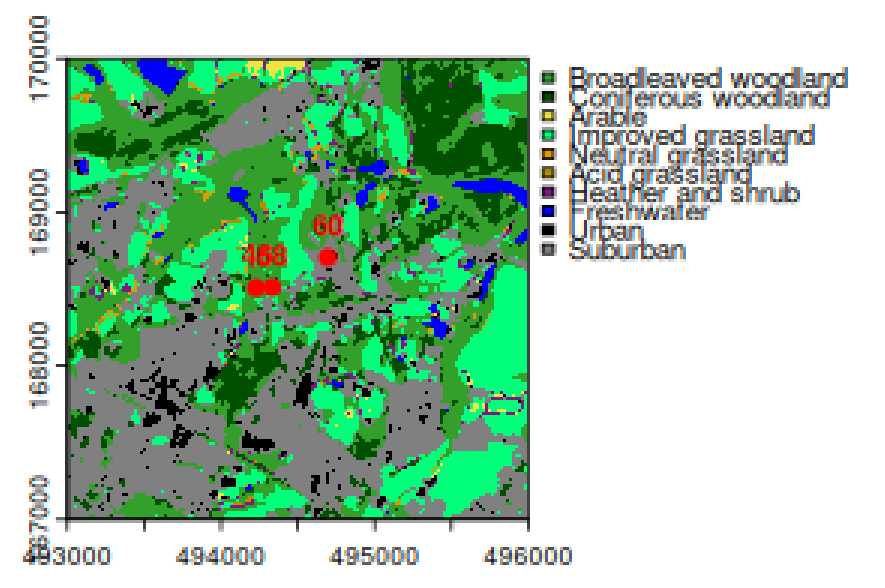
\includegraphics[width=\linewidth]{../results/location-sized.png}
    \caption{Location of the 3 selected sensors and their cover-type.}
    \label{fig:sensor_locations}
\end{figure}
\end{minipage}
\hfill
\begin{minipage}[b]{.48\textwidth}
    \centering
    \begin{table}[H]
\centering
\begin{tabular}{rllr}
  \hline
 & species & grid & n \\ 
  \hline
1 & Oryctolagus\_cuniculus & 45 &   6 \\ 
  2 & Oryctolagus\_cuniculus & 68 &   9 \\ 
  3 & Sciurus\_carolinensis & 45 &  35 \\ 
  4 & Sciurus\_carolinensis & 60 &  23 \\ 
  5 & Sciurus\_carolinensis & 68 &   3 \\ 
  6 & Vulpes\_vulpes & 60 &   1 \\ 
  7 & Vulpes\_vulpes & 68 &   8 \\ 
   \hline
\end{tabular}
\caption{Number of detections per species and sensor grid.}\label{tab:count_table}
\end{table}
\end{minipage}



\paragraph{Data analysis}
After an exploratory vizualization of species density across the NDSI gradient, I plan to use an ANOVA test to show that mean NDSI value of rabitts, squirrels and foxes habitat significantly differ, thus supporting the hypothesis that squirrels and rabbits select habitat based on anthropogenic noise levels to avoid predation risk. A Tukey HSD post-hoc test will be performed to test pairwise difference between species.

\section{Results}



\bibliography{biblio}
\end{document}